\documentclass[ignorenonframetext,]{beamer}
\usepackage{amssymb,amsmath}
\usepackage{ifxetex,ifluatex}
\usepackage{fixltx2e} % provides \textsubscript
\usepackage{lmodern}
\ifxetex
  \usepackage{fontspec,xltxtra,xunicode}
  \defaultfontfeatures{Mapping=tex-text,Scale=MatchLowercase}
  \newcommand{\euro}{€}
\else
  \ifluatex
    \usepackage{fontspec}
    \defaultfontfeatures{Mapping=tex-text,Scale=MatchLowercase}
    \newcommand{\euro}{€}
  \else
    \usepackage[T1]{fontenc}
    \usepackage[utf8]{inputenc}
      \fi
\fi
\IfFileExists{upquote.sty}{\usepackage{upquote}}{}
% use microtype if available
\IfFileExists{microtype.sty}{\usepackage{microtype}}{}
\usepackage{url}
\usepackage{letltxmacro}
\makeatletter
\def\maxwidth{\ifdim\Gin@nat@width>\linewidth\linewidth\else\Gin@nat@width\fi}
\def\maxheight{\ifdim\Gin@nat@height>\textheight0.8\textheight\else\Gin@nat@height\fi}
\makeatother
\AtBeginDocument{
  \LetLtxMacro\Oldincludegraphics\includegraphics
  \renewcommand{\includegraphics}[2][]{%
    \Oldincludegraphics[#1,width=\maxwidth,height=\maxheight,keepaspectratio]{#2}}
}

% Comment these out if you don't want a slide with just the
% part/section/subsection/subsubsection title:
\AtBeginPart{
  \let\insertpartnumber\relax
  \let\partname\relax
  \frame{\partpage}
}
\AtBeginSection{
  \let\insertsectionnumber\relax
  \let\sectionname\relax
  \frame{\sectionpage}
}
\AtBeginSubsection{
  \let\insertsubsectionnumber\relax
  \let\subsectionname\relax
  \frame{\subsectionpage}
}

\setlength{\parindent}{0pt}
\setlength{\parskip}{6pt plus 2pt minus 1pt}
\setlength{\emergencystretch}{3em}  % prevent overfull lines
\setcounter{secnumdepth}{0}

\title{Applying a biological model of the vestibulo-ocular reflex to control
gaze stabilitzation in a humanoid robot}
\author{Xavier Duran ewline, supervised by Ivan Herreros and Paul Verschure}
\date{March 25, 2015}

\begin{document}
\frame{\titlepage}

\begin{frame}{Motor learning}

\textbf{Vestibulo-ocular reflex} (VOR) adaptation is one of the most
studied cerebellar dependent motor learning tasks. It is used to provide
insight about the connections and the coding of the circuitry of the
cerebellum.

\end{frame}

\begin{frame}{Vestibulo-ocular reflex (VOR)}

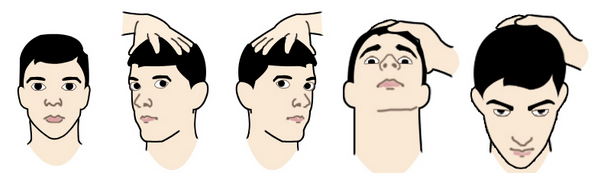
\includegraphics{images/vor.png}\footnote{\url{http://bit.ly/19GjJOA}}

This reflex functions to \textbf{stabilize images} on the retinas during
\textbf{head movement} by producing \textbf{eye movements} in the
direction opposite to head movement, thus preserving the image on the
center of the visual field.

\end{frame}

\begin{frame}{Cerebellar cortex}

\begin{itemize}
\itemsep1pt\parskip0pt\parsep0pt
\item
  Uniform structure throughout the cerebellum
\item
  Composed of repeated modules or microzones
\item
  Same cell types and connectivity
\item
  Functional units
\item
  Different inputs, different targets
\item
  Cerebellar algorithm
\end{itemize}

\end{frame}

\begin{frame}{Flocculus}

\begin{itemize}
\itemsep1pt\parskip0pt\parsep0pt
\item
  Main cerebellar region that is responsible of the control of eye
  movements
\item
  Small lobe situated on the vestibulocerebellum
\item
  Optimize ocular motor performance
\item
  Image still enough on the fovea to interpret the scene in real time
\end{itemize}

\end{frame}

\begin{frame}{Problem statement}

\begin{quote}
Computational models of the vestibulo-ocular reflex don't take into
account the role of the nucleo-olivar inhibition
\end{quote}

\end{frame}

\begin{frame}{Cerebellar microcircuit}

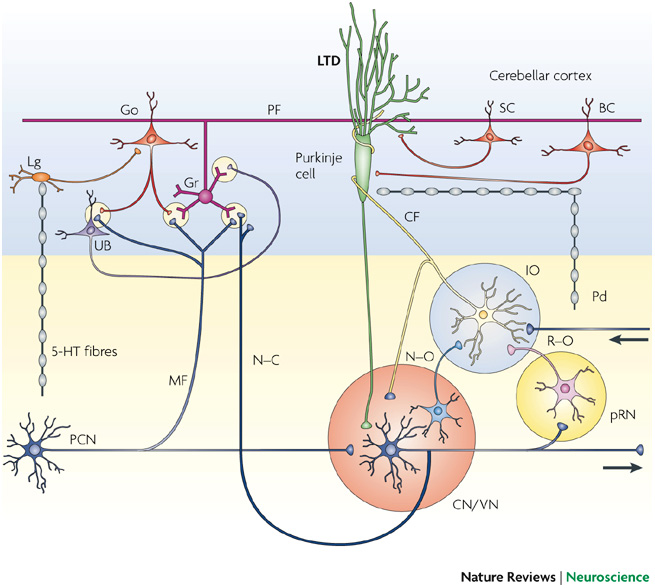
\includegraphics{images/nrn2332-f3.jpg}\footnote{\url{http://bit.ly/1AVg1qX}}

\end{frame}

\begin{frame}{Nucleo-olivary inhibition (NOI)}

On the neuroanatomical circuitries and sites of cellular plasticity
underlying adaptation of the vestibulo-ocular reflex there's a pathway
that provides feedback for adjustment of the learning instruction.

It is formed by GABAergic neurons that innervate the neurons in the
inferior olive from which the climbing fibres originate ({De Zeeuw} and
Yeo 2005)

\begin{itemize}
\itemsep1pt\parskip0pt\parsep0pt
\item
  NOI \textbf{is not} present on computational models of the VOR
\item
  NOI \textbf{is} present on \textbf{eye-blink} reflex computational
  models
\end{itemize}

\end{frame}

\begin{frame}{Trade-offs in avoidance actions}

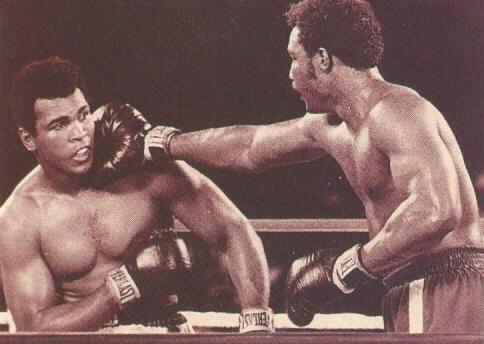
\includegraphics{images/ali.png}

\end{frame}

\begin{frame}{Extinction and NOI}

\begin{itemize}
\itemsep1pt\parskip0pt\parsep0pt
\item
  Cost-optimization
\item
  Error-based learning
\item
  Control the gain of the cerebellar output
\item
  Acquired conditioned responses are extinguished once they become no
  longer necessary
\end{itemize}

(Herreros and Verschure 2013)

\end{frame}

\begin{frame}{Research question}

What's the role of the nucleo-olivary inhibition in the vestibulo-ocular
reflex?

\begin{block}{Fingerprints}

\begin{itemize}
\itemsep1pt\parskip0pt\parsep0pt
\item
  NOI has a role in the eye-blink reflex
\item
  There is extinction of the adaptive response in the absence of
  peripheral error
\item
  VOR has a non-perfect performance, with a residual error proportional
  to the amount of cerebellar action required
\end{itemize}

(Herreros and Verschure 2013)

\end{block}

\end{frame}

\begin{frame}{Hypothesis}

Adding nucleo-olivary inhibition in the vestibulo-cerebellum explains
extinction in the state of the art vestibulo-ocular reflex computational
models.

\end{frame}

\begin{frame}{Computational models of the VOR}

Marr-Albus classical models

\end{frame}

\begin{frame}{Computational models of the VOR}

The cerebellum as an adaptive filter

\end{frame}

\begin{frame}{Computational models of the VOR}

Plasticity in the brainstem

\end{frame}

\begin{frame}{Computational models of the VOR}

A detailed model

\end{frame}

\begin{frame}{Methods}

\begin{itemize}
\itemsep1pt\parskip0pt\parsep0pt
\item
  Implementation of the detailed model (Clopath et al. 2014) of the VOR
\item
  Reproduction of the results of the paper
\item
  Add the NOI to the detailed model
\item
  Simulation of adaptation, extinction and readaptation of the VOR
\end{itemize}

\end{frame}

\begin{frame}{Implementation of the detailed model}

\begin{itemize}
\itemsep1pt\parskip0pt\parsep0pt
\item
  Simple model without delay
\item
  Simple model with delay
\item
  Detailed model
\end{itemize}

\end{frame}

\begin{frame}{Experimental setup}

\begin{columns}[T] % contents are top vertically aligned
\begin{column}[T]{5cm} % alternative top-align that's better for graphics
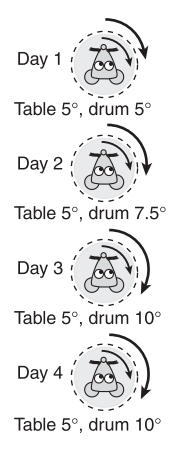
\includegraphics[height=3cm]{images/vvor.png}
\end{column}
\begin{column}[T]{5cm} % each column can also be its own environment
\begin{itemize}
\item Day 0: Normal VOR
\item Day 1: VOR cancelation (gain decrease)
\item Day 2 to 4: Phase-reversal learning
\end{itemize}
\end{column}
\end{columns}

(Wulff et al. 2009)

\end{frame}

\begin{frame}{Reproduction of the results}

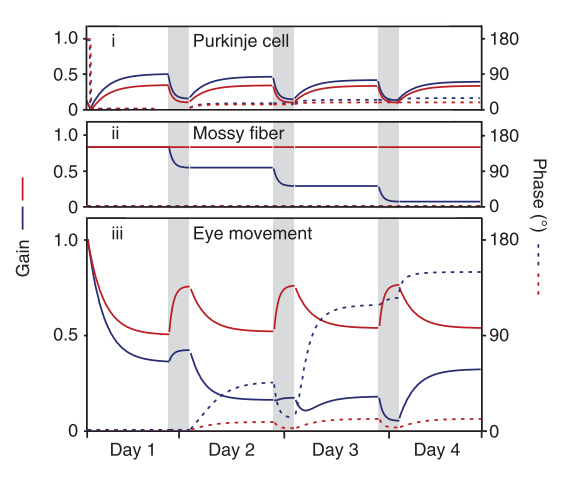
\includegraphics{images/gain.png}

(Wulff et al. 2009)

\end{frame}

\begin{frame}{Reproduction of the results}

Evolution of the gain of the VOR on the different training sessions

\begin{columns}[T]
\begin{column}[T]{5cm}
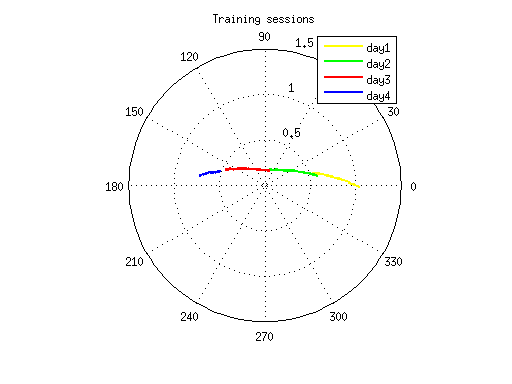
\includegraphics[height=3cm]{images/report_03.png}
\end{column}
\begin{column}[T]{5cm}
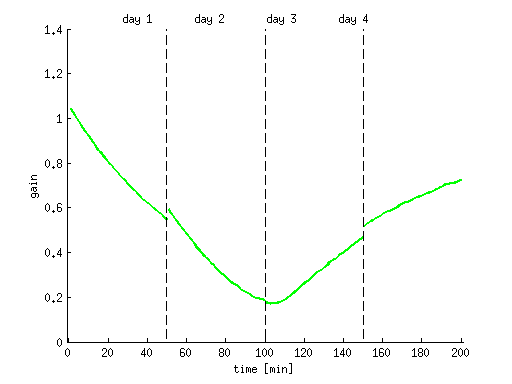
\includegraphics[height=3cm]{images/report_06.png}
\end{column}
\end{columns}

\end{frame}

\begin{frame}{Adding the NOI to the detailed mode}

Modulation in the dark of the teaching signal

\begin{itemize}
\item
  Modulated by vestibular information
  \[C(t) = \nu_{CF} - L(V(t- \delta) - V_t(t-\delta)) - H(M(t) - M_0)\]
\item
  Modulated by cortical information
  \[C(t) = \nu_{CF} - L(V(t- \delta) - V_t(t-\delta)) - H(kP(t))\]
\end{itemize}

\end{frame}

\begin{frame}{Preliminary results}

Evolution of the gain of the VOR on the different training sessions
(arbitrary \emph{k})

\begin{columns}[T]
\begin{column}[T]{5cm}
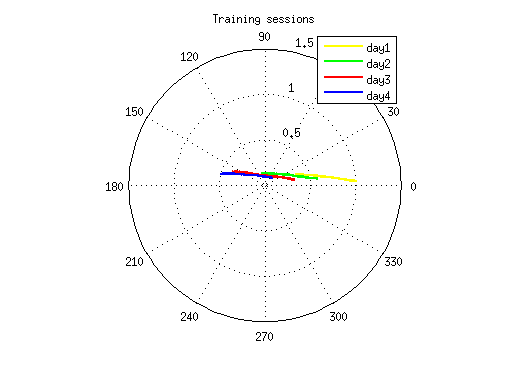
\includegraphics[height=3cm]{images/report_11.png}
\end{column}
\begin{column}[T]{5cm}
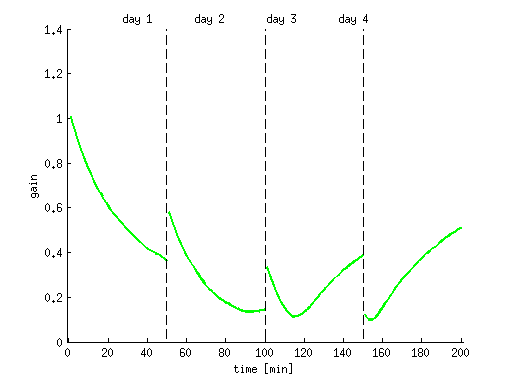
\includegraphics[height=3cm]{images/report_14.png}
\end{column}
\end{columns}

\end{frame}

\begin{frame}{Project planning}

\end{frame}

\begin{frame}{Where we are now}

\begin{itemize}
\itemsep1pt\parskip0pt\parsep0pt
\item
  Detailed model (Clopath et al. 2014) implemented in Matlab
\item
  Results reproduced as on the article
\item
  NOI added to the model
\end{itemize}

\end{frame}

\begin{frame}{Future work}

\begin{itemize}
\itemsep1pt\parskip0pt\parsep0pt
\item
  Analyze detailed model assumptions

  \begin{itemize}
  \itemsep1pt\parskip0pt\parsep0pt
  \item
    What are the effects of clipping weights on the PF-PC synapses?
  \item
    Identify other assumptions of the detailed model
  \end{itemize}
\item
  Comparing detailed and NOI models

  \begin{itemize}
  \itemsep1pt\parskip0pt\parsep0pt
  \item
    Do they show linear or exponential decay after one week light
    deprivation?
  \item
    What does maintaining the training to the cortex-nuclei memory
    balance?
  \end{itemize}
\end{itemize}

\end{frame}

\begin{frame}{References}

Clopath, Claudia, Aleksandra Badura, Chris I {De Zeeuw}, and Nicolas
Brunel. 2014. ``A Cerebellar Learning Model of Vestibulo-Ocular Reflex
Adaptation in Wild-Type and Mutant Mice.'' \emph{J. Neurosci.} 34 (21):
7203--15.
doi:\href{http://dx.doi.org/10.1523/JNEUROSCI.2791-13.2014}{10.1523/JNEUROSCI.2791-13.2014}.
\url{http://www.ncbi.nlm.nih.gov/pubmed/24849355}.

{De Zeeuw}, Chris I, and Christopher H Yeo. 2005. ``Time and Tide in
Cerebellar Memory Formation.'' \emph{Curr. Opin. Neurobiol.} 15 (6):
667--74.
doi:\href{http://dx.doi.org/10.1016/j.conb.2005.10.008}{10.1016/j.conb.2005.10.008}.
\url{http://www.ncbi.nlm.nih.gov/pubmed/16271462}.

Herreros, Ivan, and Paul F M J Verschure. 2013. ``Nucleo-Olivary
Inhibition Balances the Interaction Between the Reactive and Adaptive
Layers in Motor Control.'' \emph{Neural Netw.} 47 (November). Elsevier
Ltd: 64--71.
doi:\href{http://dx.doi.org/10.1016/j.neunet.2013.01.026}{10.1016/j.neunet.2013.01.026}.
\url{http://www.ncbi.nlm.nih.gov/pubmed/23535576}.

Wulff, Peer, Martijn Schonewille, Massimiliano Renzi, Laura Viltono,
Marco Sassoè-Pognetto, Aleksandra Badura, Zhenyu Gao, et al. 2009.
``Synaptic Inhibition of Purkinje Cells Mediates Consolidation of
Vestibulo-Cerebellar Motor Learning.'' \emph{Nat. Neurosci.} 12 (8):
1042--9. doi:\href{http://dx.doi.org/10.1038/nn.2348}{10.1038/nn.2348}.
\url{http://www.pubmedcentral.nih.gov/articlerender.fcgi?artid=2718327/\&tool=pmcentrez/\&rendertype=abstract}.

\end{frame}

\end{document}
